\chapter{Proposed Syntactic and Semantic Analyser}
\label{ch:proposed-sin-sema-anal}
After analysing the existing tools, we can see that different
aspects of existing technology can be improved, such as those
discussed in \cref{sec:anal-enhacements}. In this chapter we
model a proposal by means of software engineering techniques.

Within these techniques, the process we are going to follow
to model the proposal is first obtain the use cases through
the possible improvements detected in the previous chapter.
From these use cases we will extract the requirements. Once
the requirements have been extracted, we will proceed to
design the solution using diagrams.

We know that the system will be composed of at least a lexical
analyser, a syntactic analyser, a semantic analyser and some
type of message manager to handle errors and warnings.

\section{Error Handler}
Of the improvements that we observe in \cref{sec:anal-enhacements}, those
that have to do with the error / warning management
system are 1, 2 and 6. The following diagram considers
these use cases in the error / warning management system.

\begin{figure}[h!]
    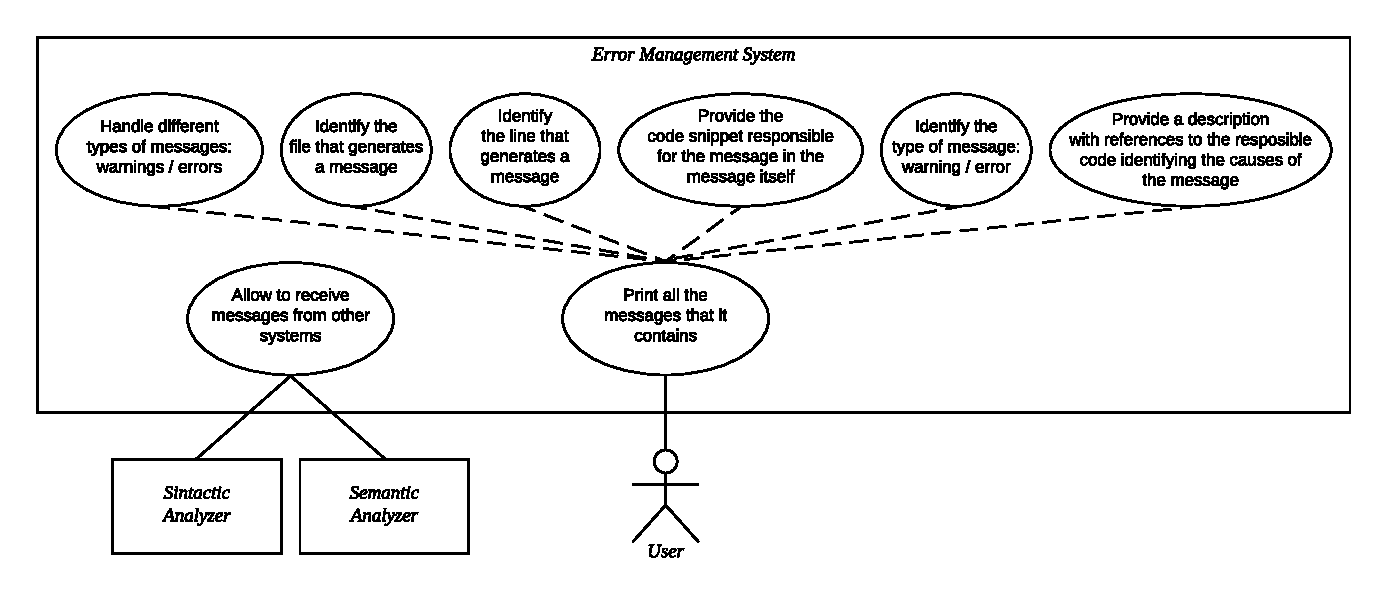
\includegraphics[scale=0.6]{images/err-hand-use-case.pdf}
    \centering
    \caption[Error handler use cases]{Error handler use cases.}
    \label{fig:err-hand-use-case}
\end{figure}

Thus, from the use cases mentioned in the previous section we
extract the following functional requirements.

\begin{figure}[h!]
    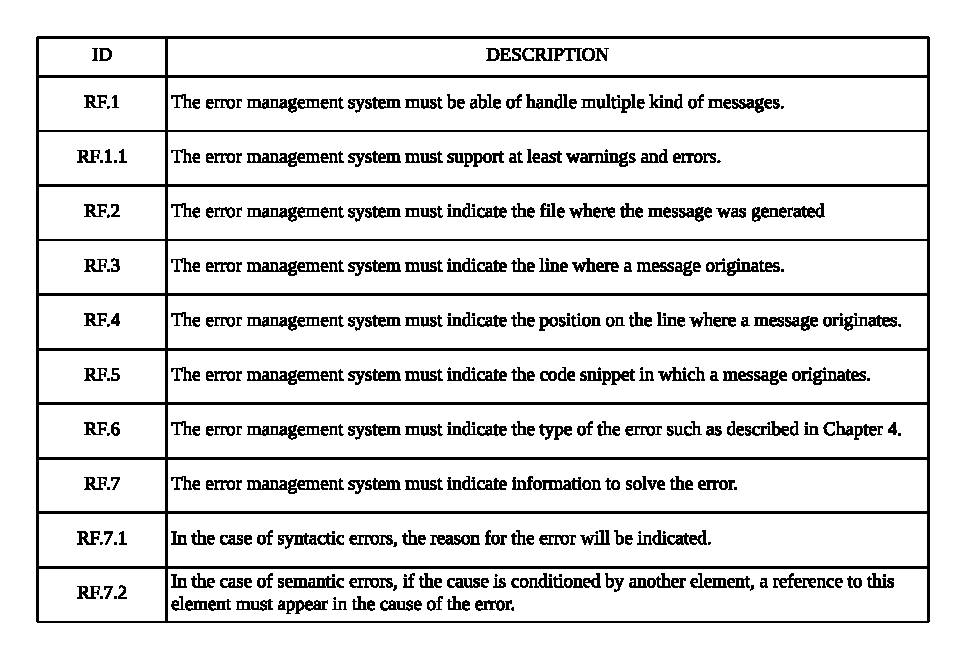
\includegraphics[width=\textwidth]{images/err-hand-reqf.pdf}
    \centering
    \caption[Error handler functional requirements]{Error handler functional requirements.}
    \label{fig:err-hand-reqf}
\end{figure}

From the use cases we can also extract the following interface requirements.

\begin{figure}[h!]
    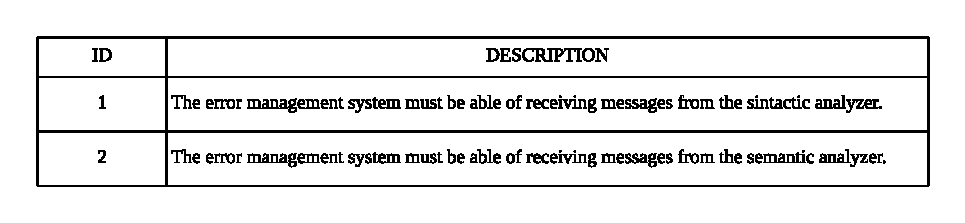
\includegraphics[width=\textwidth]{images/err-hand-reqnf.pdf}
    \centering
    \caption[Error handler non functional requirements]{Error handler non functional requirements.}
    \label{fig:err-hand-reqnf}
\end{figure}

For the previous requirements we propose the following diagram for the error management system (\cref{fig:err-hand-diag}).

\begin{figure}[h!]
    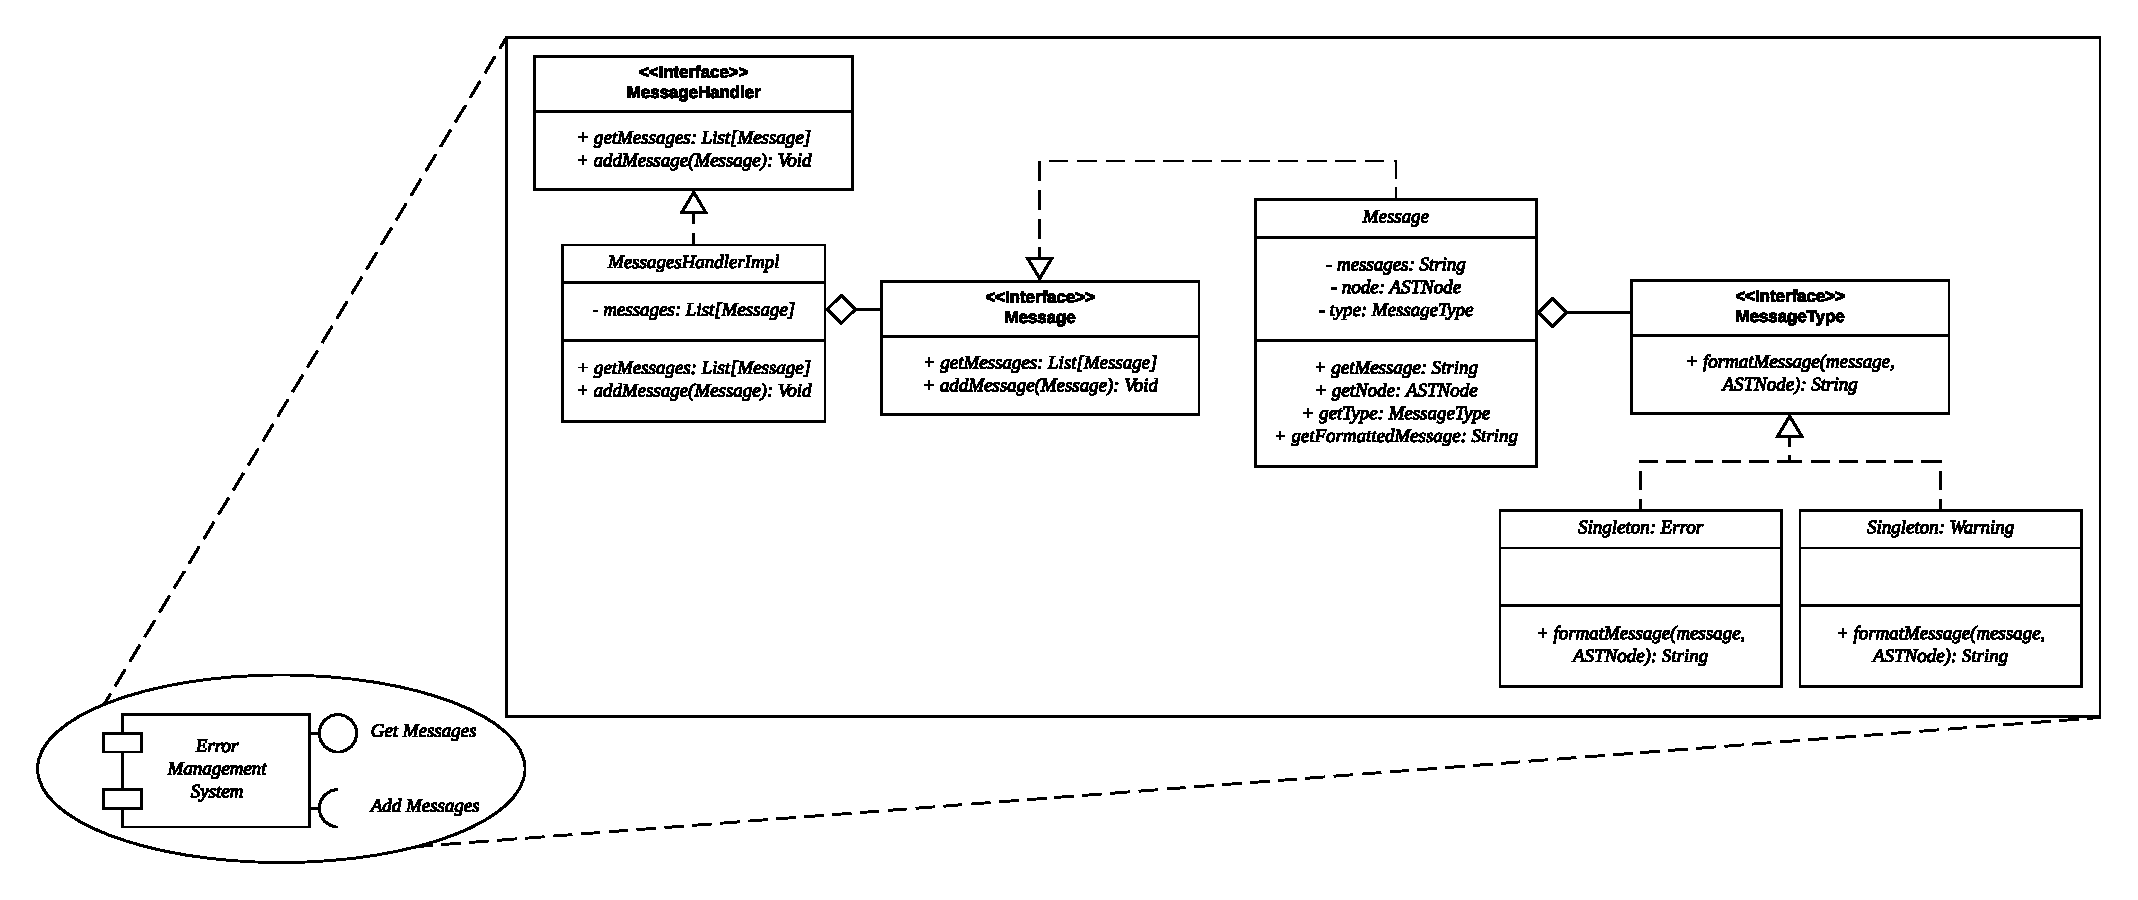
\includegraphics[width=\textwidth]{images/err-hand-diagram.pdf}
    \centering
    \caption[Error handler component and class diagrams]{Error handler component and class diagrams.}
    \label{fig:err-hand-diag}
\end{figure}


\section{Lexical Analyser}
The lexical analyser is necessary to subsequently carry out syntactic and semantic analysis.
And therefore, although it is not contemplated as an improvement in
the previous chapter, we do have to include it in our proposed system. The following diagram
shows the expected use cases of a lexical analyser in our context.

\begin{figure}[h!]
    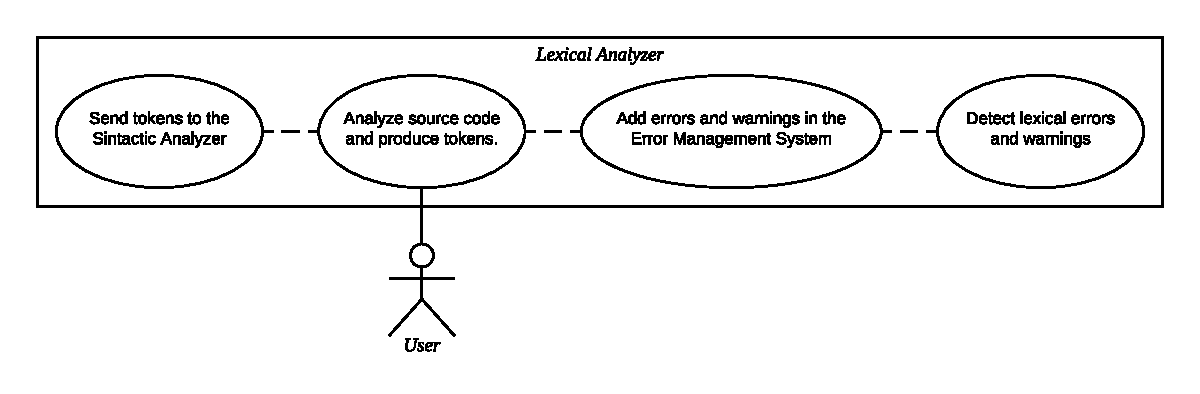
\includegraphics[scale=0.6]{images/lex-use-case.pdf}
    \centering
    \caption[Lexical analyser use cases]{Lexical analyser use cases.}
    \label{fig:lex-use-case}
\end{figure}

Thus, from the use cases mentioned in the previous section we
extract the following functional requirements.

\begin{figure}[h!]
    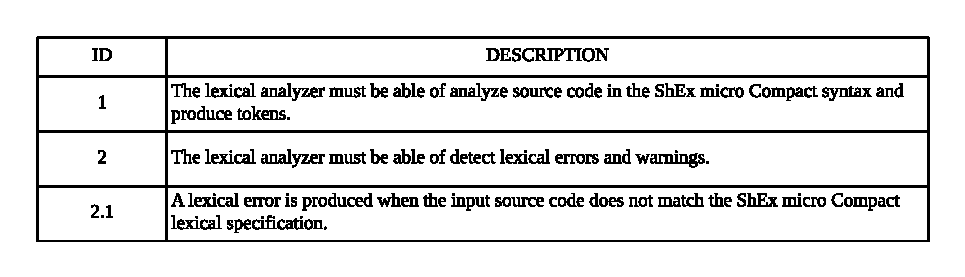
\includegraphics[width=\textwidth]{images/lex-reqf.pdf}
    \centering
    \caption[Lexical analyser functional requirements]{Lexical analyser functional requirements.}
    \label{fig:lex-reqf}
\end{figure}

From the use cases we can also extract the following interface requirements.

\begin{figure}[h!]
    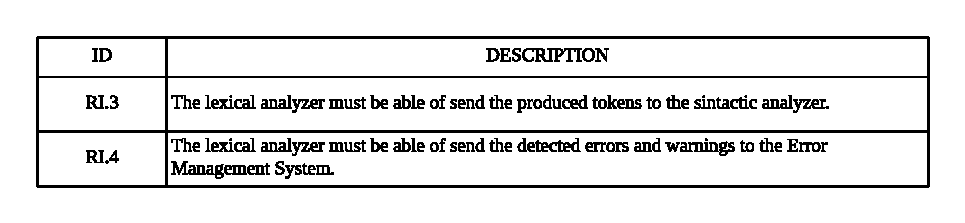
\includegraphics[width=\textwidth]{images/lex-reqnf.pdf}
    \centering
    \caption[Lexical analyser non functional requirements]{Lexical analyser non functional requirements.}
    \label{fig:lex-reqnf}
\end{figure}

For the previous requirements we propose the following model for the lexical analyser.

\begin{figure}[h!]
    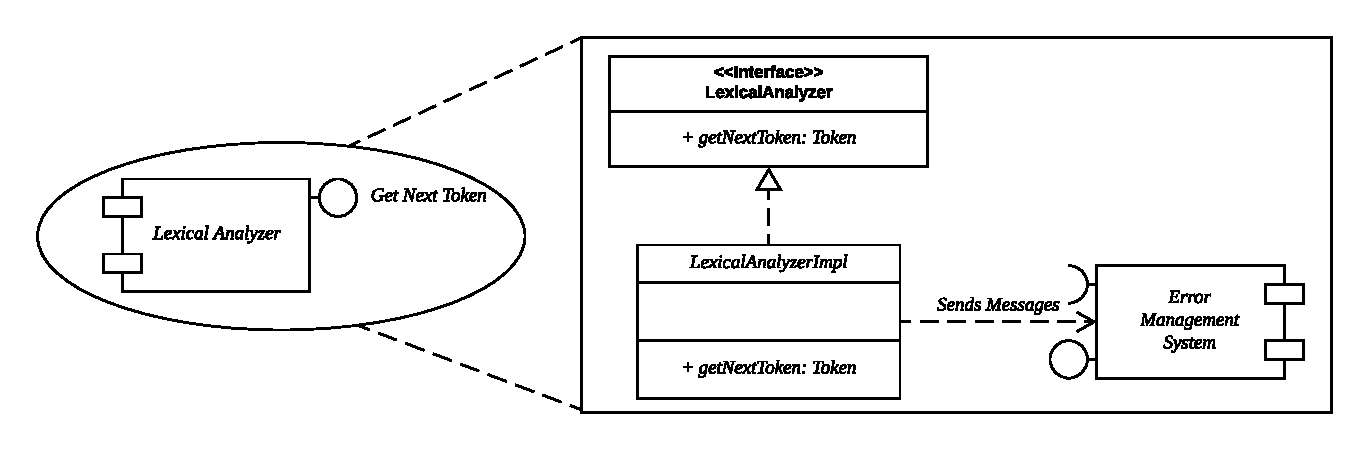
\includegraphics[width=\textwidth]{images/lex-diagram.pdf}
    \centering
    \caption[Lexical analyser component and class diagrams]{Lexical analyser component and class diagrams.}
    \label{fig:lex-diag}
\end{figure}

\section{Syntactic Analyser}
The parser may not be so necessary if we are looking to improve existing systems, but it is
necessary to carry out the next step, semantic analysis. To others
in this step you can also propose some improvement, although less. The following diagram
shows the expected use cases for a system that wants to implement a syntactic validator.

\begin{figure}[h!]
    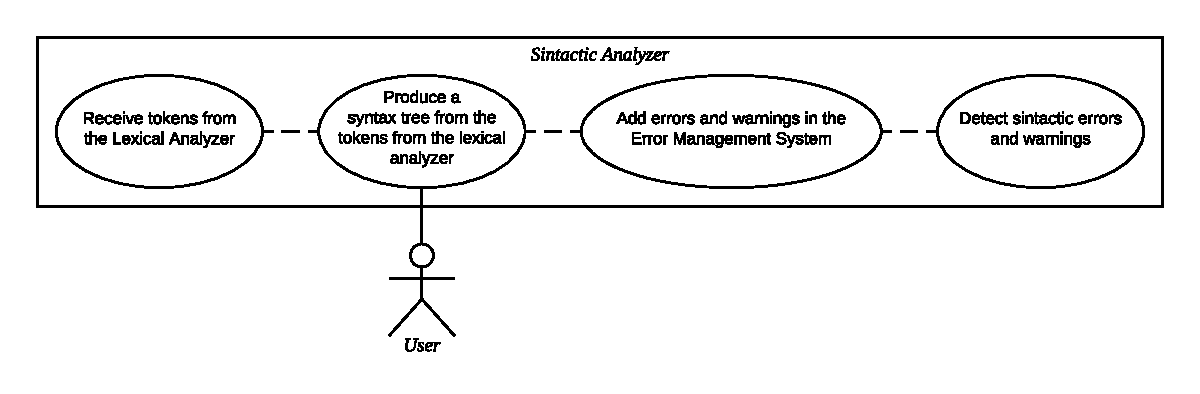
\includegraphics[scale=0.6]{images/sin-use-case.pdf}
    \centering
    \caption[Syntactic analyser use cases]{Syntactic analyser use cases.}
    \label{fig:sin-use-case}
\end{figure}

Thus, from the use cases mentioned in the previous section we
extract the following functional requirements.

\begin{figure}[h!]
    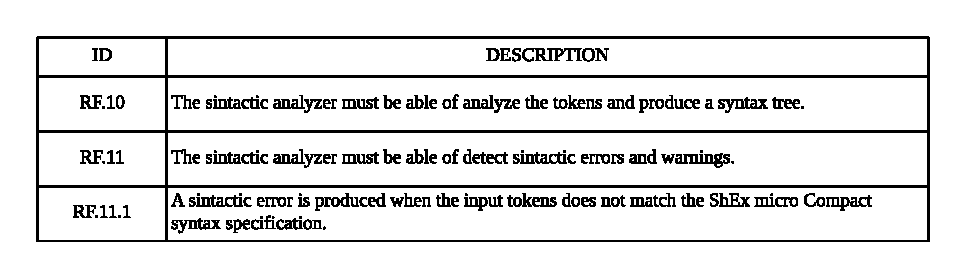
\includegraphics[width=\textwidth]{images/sin-reqf.pdf}
    \centering
    \caption[Syntactic analyser functional requirements]{Syntactic analyser functional requirements.}
    \label{fig:sin-reqf}
\end{figure}

From the use cases we can also extract the following interface requirements.

\begin{figure}[h!]
    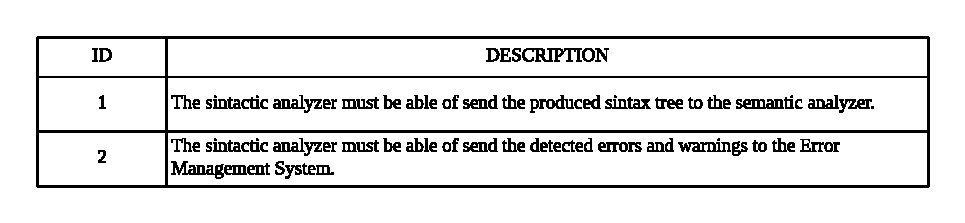
\includegraphics[width=\textwidth]{images/sin-reqnf.pdf}
    \centering
    \caption[Syntactic analyser non functional requirements]{Syntactic analyser non functional requirements.}
    \label{fig:sin-reqnf}
\end{figure}

For the previous requirements we propose the following modulation for the syntactic analyser.

\begin{figure}[h!]
    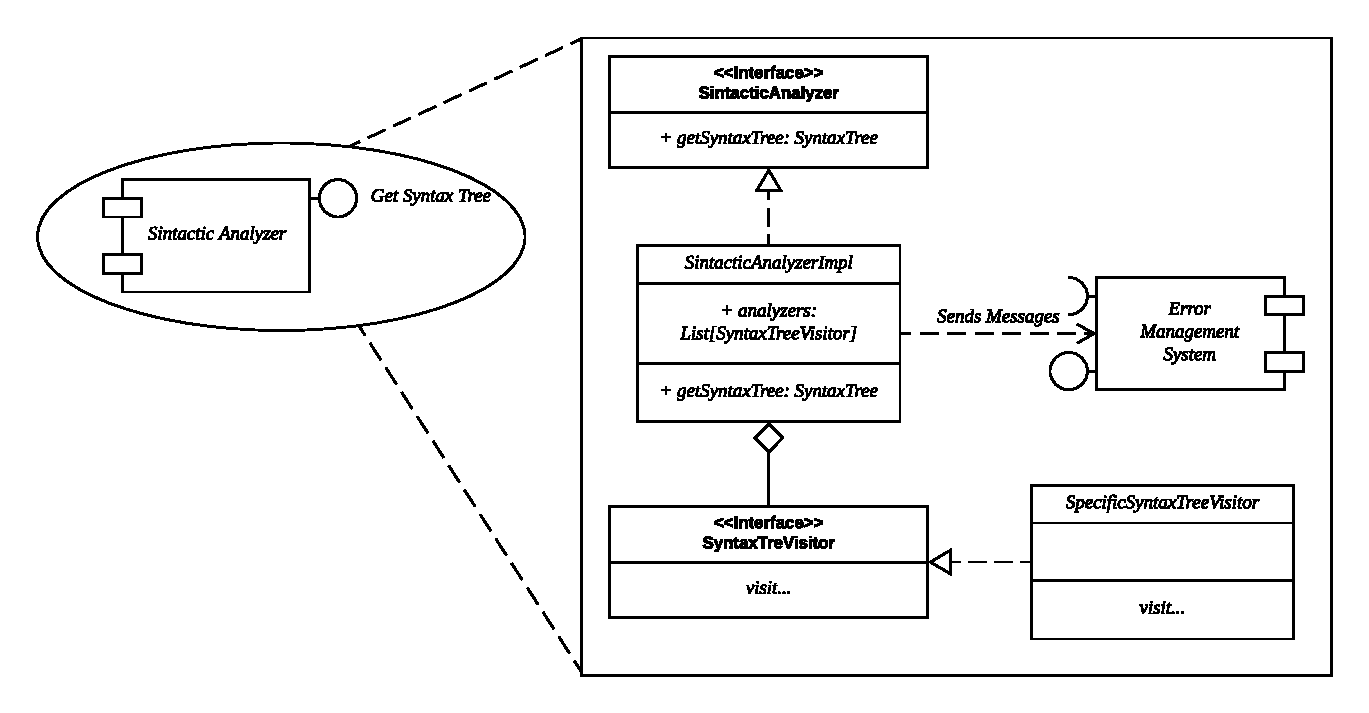
\includegraphics[width=\textwidth]{images/sin-diagram.pdf}
    \centering
    \caption[Syntactic analyser component and class diagrams]{Syntactic analyser component and class diagrams.}
    \label{fig:sin-diag}
\end{figure}

\section{Semantic Analyser}
The semantic analyser is key in our architecture since most of the improvements
that have to do with finding new types of errors can be identified through semantic
validations. The following diagram shows the expected use cases for a system that
wants to implement a semantic validator to solve the above problems.

\begin{figure}[h!]
    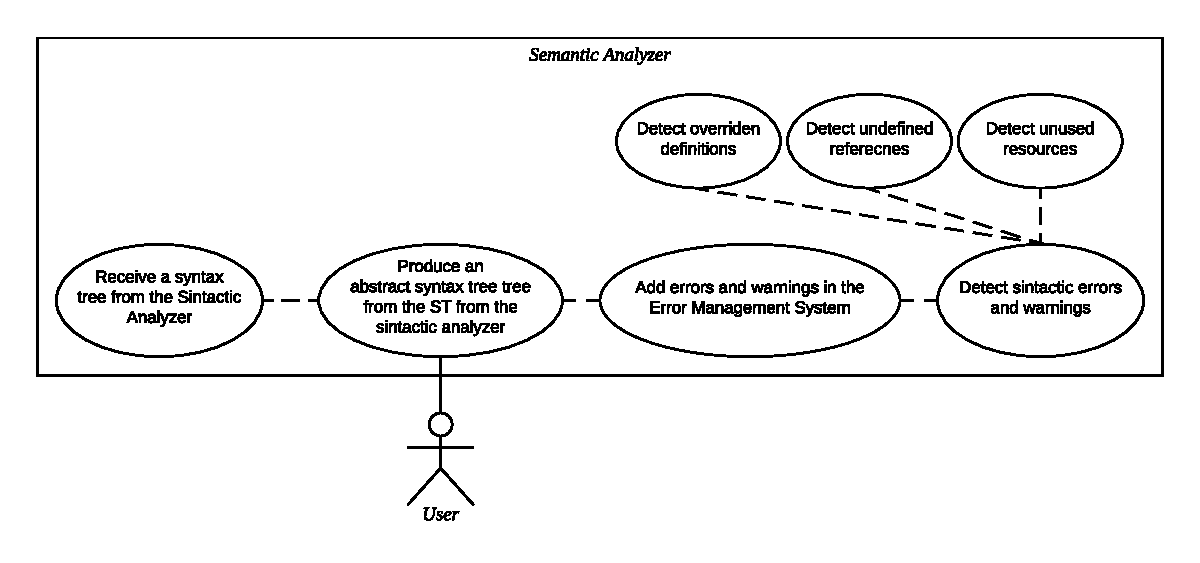
\includegraphics[scale=0.6]{images/sema-use-case.pdf}
    \centering
    \caption[Semantic analyser use cases]{Semantic analyser use cases.}
    \label{fig:sema-use-case}
\end{figure}

Thus, from the use cases mentioned in the previous section we
extract the following functional requirements.

\begin{figure}[h!]
    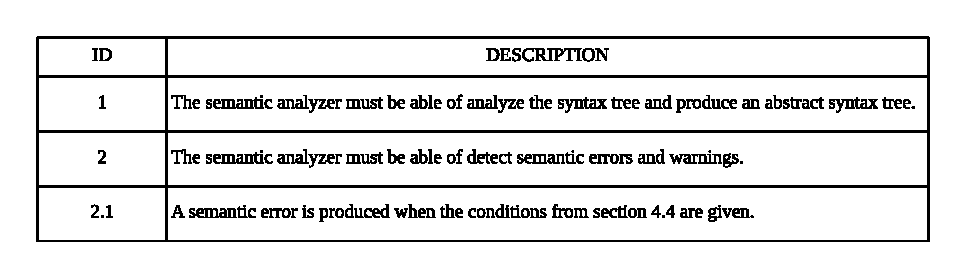
\includegraphics[width=\textwidth]{images/sema-reqf.pdf}
    \centering
    \caption[Semantic analyser functional requirements]{Semantic analyser functional requirements.}
    \label{fig:sema-reqf}
\end{figure}

From the use cases we can also extract the following interface requirements.

\begin{figure}[h!]
    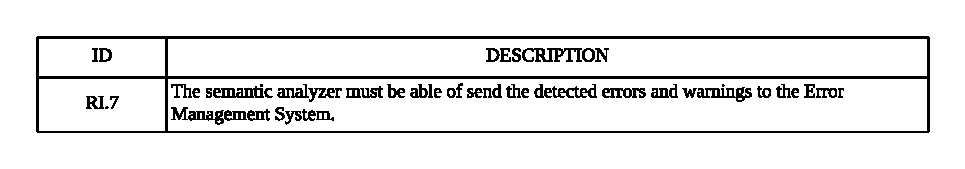
\includegraphics[width=\textwidth]{images/sema-reqnf.pdf}
    \centering
    \caption[Semantic analyser non functional requirements]{Semantic analyser non functional requirements.}
    \label{fig:sema-reqnf}
\end{figure}

For the previous requirements we propose the following model for the semantic analyser.

\begin{figure}[h!]
    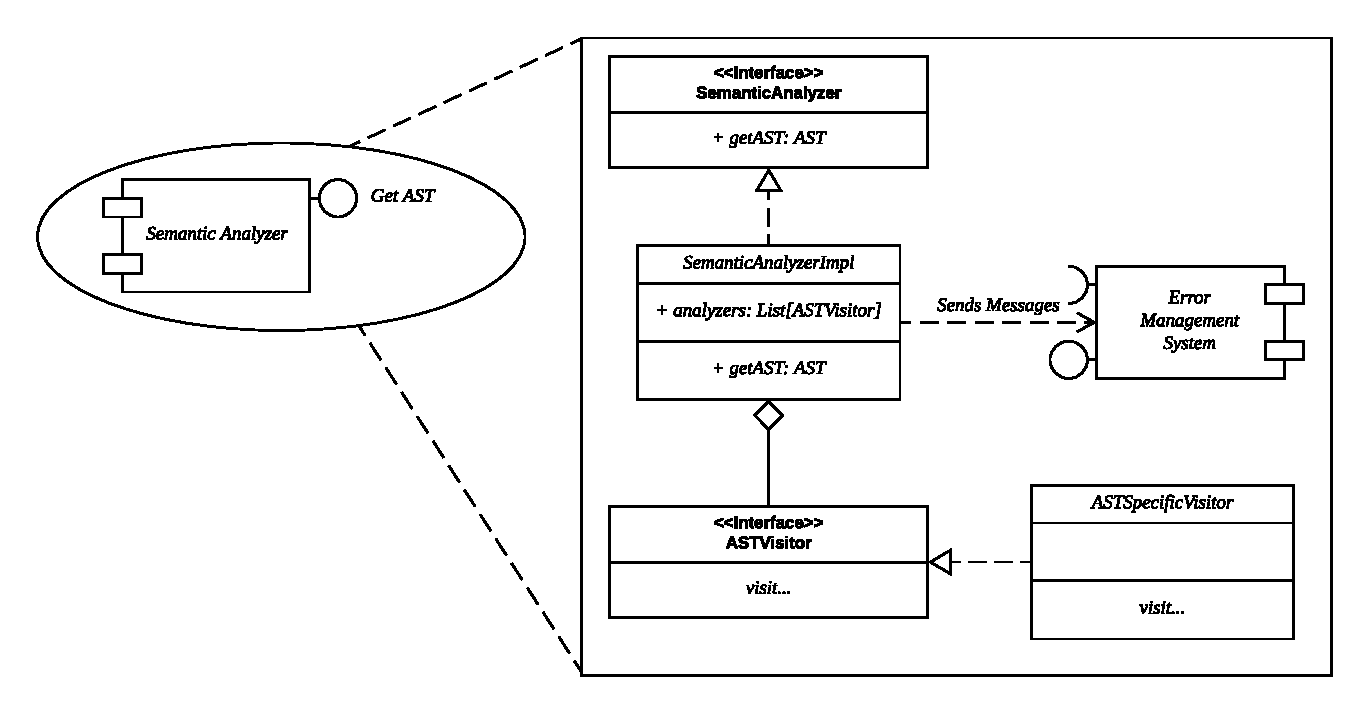
\includegraphics[width=\textwidth]{images/sema-diagram.pdf}
    \centering
    \caption[Semantic analyser component and class diagrams]{Semantic analyser component and class diagrams.}
    \label{fig:sema-diag}
\end{figure}

\section{Full System Diagram}
After analysing and designing each component now we offer a
complete view of the entire integrated system. In addition
you can see that a new component appears, the symbol table.
This component can be any type of structure that fulfils the
expected basic functions of a symbol table.

\begin{figure}[h!]
    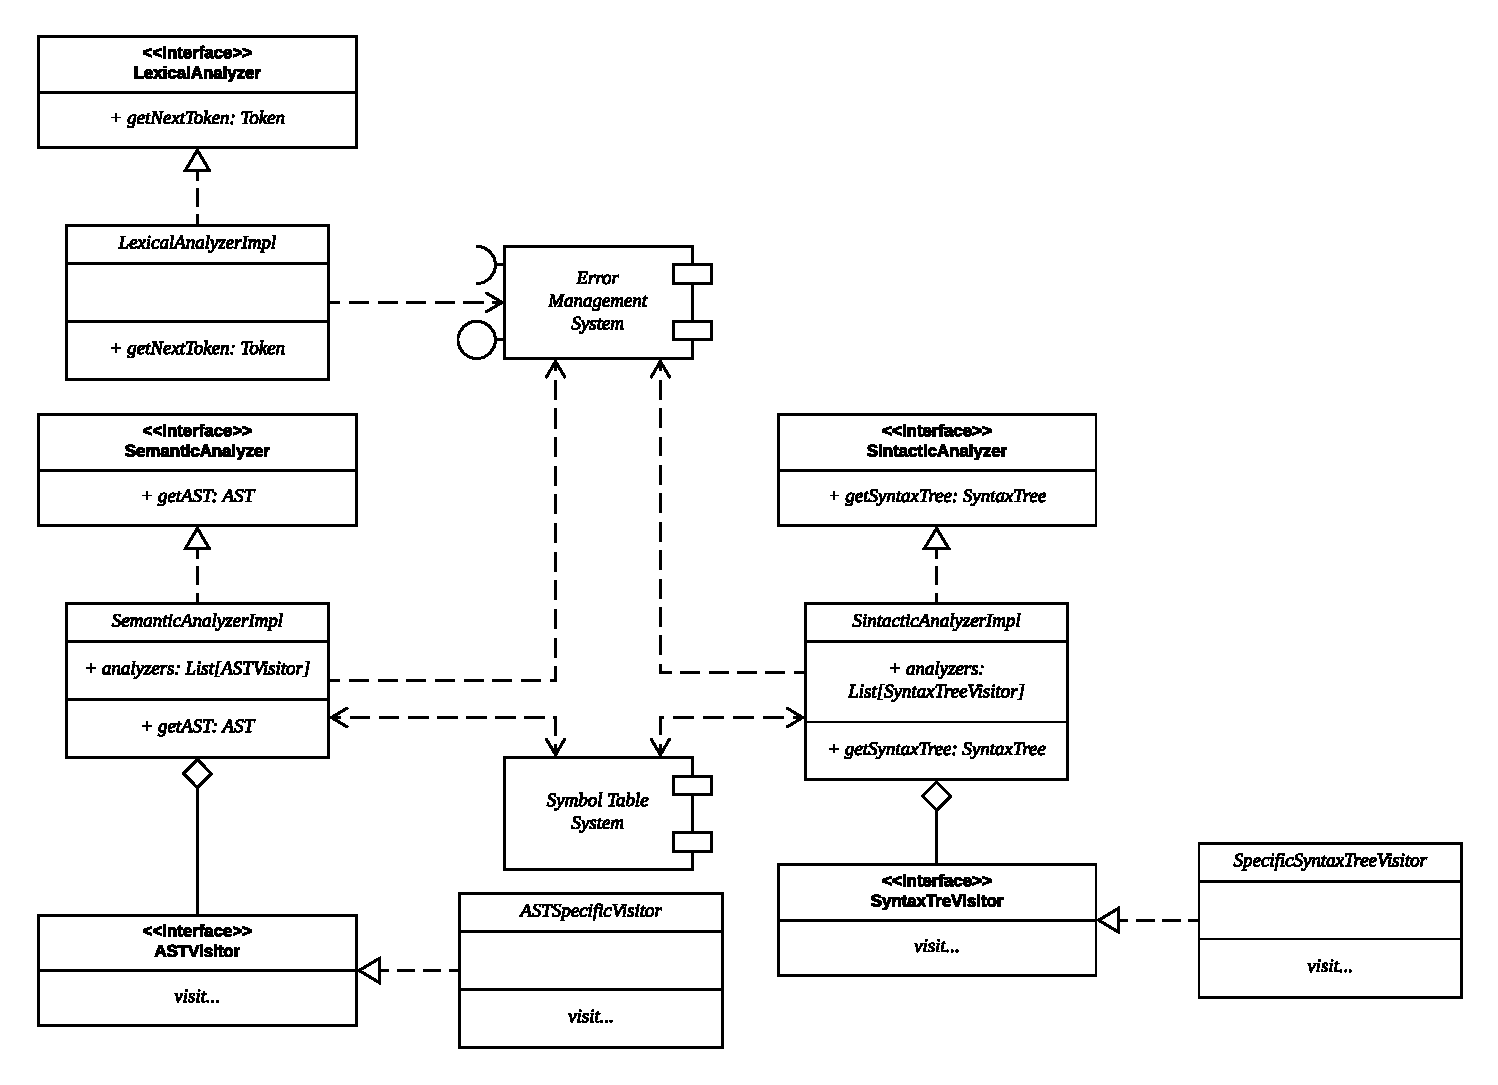
\includegraphics[scale=0.4]{images/full-diagram.pdf}
    \centering
    \caption[Complete system class diagram]{Complete system class diagram.}
    \label{fig:full-diag}
\end{figure}